\section{Per-seed results}
\label{supp:seeds}
Table~\ref{tab:seeds} lists every run behind the headline comparison, with the mean and sample standard deviation over seeds. Table~\ref{tab:seedmargin} gives the per-seed mAP margin of v2 over the concat baseline, which is the quantity averaged in Table~I of the main paper.

\begin{table*}[t]
\centering
\caption{Per-seed accuracy in percent, 80 epochs. The last three columns are COCO size bands.}
\label{tab:seeds}
{\footnotesize\setlength{\tabcolsep}{4.5pt}
\begin{tabular}{llcccccccc}
\toprule
Dataset & Model & Seed & mAP & mAP$_{50}$ & Precision & Recall & Small & Medium & Large \\
\midrule
LLVIP & Concat, modality dropout & 0 & \resLlvipConcatMdSeedZeroMap & \resLlvipConcatMdSeedZeroMapFifty & \resLlvipConcatMdSeedZeroPrecision & \resLlvipConcatMdSeedZeroRecall & \resLlvipConcatMdSeedZeroApSmall & \resLlvipConcatMdSeedZeroApMedium & \resLlvipConcatMdSeedZeroApLarge \\
 &  & 1 & \resLlvipConcatMdSeedOneMap & \resLlvipConcatMdSeedOneMapFifty & \resLlvipConcatMdSeedOnePrecision & \resLlvipConcatMdSeedOneRecall & \resLlvipConcatMdSeedOneApSmall & \resLlvipConcatMdSeedOneApMedium & \resLlvipConcatMdSeedOneApLarge \\
 &  & 2 & \resLlvipConcatMdSeedTwoMap & \resLlvipConcatMdSeedTwoMapFifty & \resLlvipConcatMdSeedTwoPrecision & \resLlvipConcatMdSeedTwoRecall & \resLlvipConcatMdSeedTwoApSmall & \resLlvipConcatMdSeedTwoApMedium & \resLlvipConcatMdSeedTwoApLarge \\
& \emph{mean $\pm$ std} & & \resLlvipConcatMdMeanMap\,\ensuremath{\pm}\,\resLlvipConcatMdStdMap & \resLlvipConcatMdMeanMapFifty\,\ensuremath{\pm}\,\resLlvipConcatMdStdMapFifty & \resLlvipConcatMdMeanPrecision\,\ensuremath{\pm}\,\resLlvipConcatMdStdPrecision & \resLlvipConcatMdMeanRecall\,\ensuremath{\pm}\,\resLlvipConcatMdStdRecall & \resLlvipConcatMdMeanApSmall\,\ensuremath{\pm}\,\resLlvipConcatMdStdApSmall & \resLlvipConcatMdMeanApMedium\,\ensuremath{\pm}\,\resLlvipConcatMdStdApMedium & \resLlvipConcatMdMeanApLarge\,\ensuremath{\pm}\,\resLlvipConcatMdStdApLarge \\
 & CFFM-Net v2 & 0 & \resLlvipCffmVtwoSeedZeroMap & \resLlvipCffmVtwoSeedZeroMapFifty & \resLlvipCffmVtwoSeedZeroPrecision & \resLlvipCffmVtwoSeedZeroRecall & \resLlvipCffmVtwoSeedZeroApSmall & \resLlvipCffmVtwoSeedZeroApMedium & \resLlvipCffmVtwoSeedZeroApLarge \\
 &  & 1 & \resLlvipCffmVtwoSeedOneMap & \resLlvipCffmVtwoSeedOneMapFifty & \resLlvipCffmVtwoSeedOnePrecision & \resLlvipCffmVtwoSeedOneRecall & \resLlvipCffmVtwoSeedOneApSmall & \resLlvipCffmVtwoSeedOneApMedium & \resLlvipCffmVtwoSeedOneApLarge \\
 &  & 2 & \resLlvipCffmVtwoSeedTwoMap & \resLlvipCffmVtwoSeedTwoMapFifty & \resLlvipCffmVtwoSeedTwoPrecision & \resLlvipCffmVtwoSeedTwoRecall & \resLlvipCffmVtwoSeedTwoApSmall & \resLlvipCffmVtwoSeedTwoApMedium & \resLlvipCffmVtwoSeedTwoApLarge \\
& \emph{mean $\pm$ std} & & \resLlvipCffmVtwoMeanMap\,\ensuremath{\pm}\,\resLlvipCffmVtwoStdMap & \resLlvipCffmVtwoMeanMapFifty\,\ensuremath{\pm}\,\resLlvipCffmVtwoStdMapFifty & \resLlvipCffmVtwoMeanPrecision\,\ensuremath{\pm}\,\resLlvipCffmVtwoStdPrecision & \resLlvipCffmVtwoMeanRecall\,\ensuremath{\pm}\,\resLlvipCffmVtwoStdRecall & \resLlvipCffmVtwoMeanApSmall\,\ensuremath{\pm}\,\resLlvipCffmVtwoStdApSmall & \resLlvipCffmVtwoMeanApMedium\,\ensuremath{\pm}\,\resLlvipCffmVtwoStdApMedium & \resLlvipCffmVtwoMeanApLarge\,\ensuremath{\pm}\,\resLlvipCffmVtwoStdApLarge \\
\midrule
M3FD & Concat, modality dropout & 0 & \resMfdConcatMdSeedZeroMap & \resMfdConcatMdSeedZeroMapFifty & \resMfdConcatMdSeedZeroPrecision & \resMfdConcatMdSeedZeroRecall & \resMfdConcatMdSeedZeroApSmall & \resMfdConcatMdSeedZeroApMedium & \resMfdConcatMdSeedZeroApLarge \\
 &  & 1 & \resMfdConcatMdSeedOneMap & \resMfdConcatMdSeedOneMapFifty & \resMfdConcatMdSeedOnePrecision & \resMfdConcatMdSeedOneRecall & \resMfdConcatMdSeedOneApSmall & \resMfdConcatMdSeedOneApMedium & \resMfdConcatMdSeedOneApLarge \\
 &  & 2 & \resMfdConcatMdSeedTwoMap & \resMfdConcatMdSeedTwoMapFifty & \resMfdConcatMdSeedTwoPrecision & \resMfdConcatMdSeedTwoRecall & \resMfdConcatMdSeedTwoApSmall & \resMfdConcatMdSeedTwoApMedium & \resMfdConcatMdSeedTwoApLarge \\
& \emph{mean $\pm$ std} & & \resMfdConcatMdMeanMap\,\ensuremath{\pm}\,\resMfdConcatMdStdMap & \resMfdConcatMdMeanMapFifty\,\ensuremath{\pm}\,\resMfdConcatMdStdMapFifty & \resMfdConcatMdMeanPrecision\,\ensuremath{\pm}\,\resMfdConcatMdStdPrecision & \resMfdConcatMdMeanRecall\,\ensuremath{\pm}\,\resMfdConcatMdStdRecall & \resMfdConcatMdMeanApSmall\,\ensuremath{\pm}\,\resMfdConcatMdStdApSmall & \resMfdConcatMdMeanApMedium\,\ensuremath{\pm}\,\resMfdConcatMdStdApMedium & \resMfdConcatMdMeanApLarge\,\ensuremath{\pm}\,\resMfdConcatMdStdApLarge \\
 & CFFM-Net v2 & 0 & \resMfdCffmVtwoSeedZeroMap & \resMfdCffmVtwoSeedZeroMapFifty & \resMfdCffmVtwoSeedZeroPrecision & \resMfdCffmVtwoSeedZeroRecall & \resMfdCffmVtwoSeedZeroApSmall & \resMfdCffmVtwoSeedZeroApMedium & \resMfdCffmVtwoSeedZeroApLarge \\
 &  & 1 & \resMfdCffmVtwoSeedOneMap & \resMfdCffmVtwoSeedOneMapFifty & \resMfdCffmVtwoSeedOnePrecision & \resMfdCffmVtwoSeedOneRecall & \resMfdCffmVtwoSeedOneApSmall & \resMfdCffmVtwoSeedOneApMedium & \resMfdCffmVtwoSeedOneApLarge \\
 &  & 2 & \resMfdCffmVtwoSeedTwoMap & \resMfdCffmVtwoSeedTwoMapFifty & \resMfdCffmVtwoSeedTwoPrecision & \resMfdCffmVtwoSeedTwoRecall & \resMfdCffmVtwoSeedTwoApSmall & \resMfdCffmVtwoSeedTwoApMedium & \resMfdCffmVtwoSeedTwoApLarge \\
& \emph{mean $\pm$ std} & & \resMfdCffmVtwoMeanMap\,\ensuremath{\pm}\,\resMfdCffmVtwoStdMap & \resMfdCffmVtwoMeanMapFifty\,\ensuremath{\pm}\,\resMfdCffmVtwoStdMapFifty & \resMfdCffmVtwoMeanPrecision\,\ensuremath{\pm}\,\resMfdCffmVtwoStdPrecision & \resMfdCffmVtwoMeanRecall\,\ensuremath{\pm}\,\resMfdCffmVtwoStdRecall & \resMfdCffmVtwoMeanApSmall\,\ensuremath{\pm}\,\resMfdCffmVtwoStdApSmall & \resMfdCffmVtwoMeanApMedium\,\ensuremath{\pm}\,\resMfdCffmVtwoStdApMedium & \resMfdCffmVtwoMeanApLarge\,\ensuremath{\pm}\,\resMfdCffmVtwoStdApLarge \\
\bottomrule
\end{tabular}}
\end{table*}

\begin{table}[t]
\centering
\caption{Per-seed mAP margin of CFFM-Net v2 over the concat baseline, in percentage points.}
\label{tab:seedmargin}
{\footnotesize\setlength{\tabcolsep}{6pt}
\begin{tabular}{lccc}
\toprule
Dataset & Seed 0 & Seed 1 & Seed 2 \\
\midrule
LLVIP & \marLlvipVtwoVsConcatMdSeedZeroMap & \marLlvipVtwoVsConcatMdSeedOneMap & \marLlvipVtwoVsConcatMdSeedTwoMap \\
M3FD & \marMfdVtwoVsConcatMdSeedZeroMap & \marMfdVtwoVsConcatMdSeedOneMap & \marMfdVtwoVsConcatMdSeedTwoMap \\
\bottomrule
\end{tabular}}
\end{table}

\section{Fine size bands on M3FD}
\label{supp:bands}
Table~\ref{tab:bands} gives the finer size bands behind the small-object analysis of the main paper.

\begin{table}[t]
\centering
\caption{M3FD average precision in the finer size bands, percent, per seed and as mean and sample standard deviation.}
\label{tab:bands}
{\footnotesize\setlength{\tabcolsep}{3.5pt}
\begin{tabular}{llccc}
\toprule
Model & Seed & Very tiny & Tiny & Small \\
\midrule
Concat, modality dropout & 0 & \resMfdConcatMdSeedZeroApBandVeryTiny & \resMfdConcatMdSeedZeroApBandTiny & \resMfdConcatMdSeedZeroApBandSmall \\
 & 1 & \resMfdConcatMdSeedOneApBandVeryTiny & \resMfdConcatMdSeedOneApBandTiny & \resMfdConcatMdSeedOneApBandSmall \\
 & 2 & \resMfdConcatMdSeedTwoApBandVeryTiny & \resMfdConcatMdSeedTwoApBandTiny & \resMfdConcatMdSeedTwoApBandSmall \\
& \emph{mean $\pm$ std} & \resMfdConcatMdMeanApBandVeryTiny\,\ensuremath{\pm}\,\resMfdConcatMdStdApBandVeryTiny & \resMfdConcatMdMeanApBandTiny\,\ensuremath{\pm}\,\resMfdConcatMdStdApBandTiny & \resMfdConcatMdMeanApBandSmall\,\ensuremath{\pm}\,\resMfdConcatMdStdApBandSmall \\
\midrule
CFFM-Net v2 & 0 & \resMfdCffmVtwoSeedZeroApBandVeryTiny & \resMfdCffmVtwoSeedZeroApBandTiny & \resMfdCffmVtwoSeedZeroApBandSmall \\
 & 1 & \resMfdCffmVtwoSeedOneApBandVeryTiny & \resMfdCffmVtwoSeedOneApBandTiny & \resMfdCffmVtwoSeedOneApBandSmall \\
 & 2 & \resMfdCffmVtwoSeedTwoApBandVeryTiny & \resMfdCffmVtwoSeedTwoApBandTiny & \resMfdCffmVtwoSeedTwoApBandSmall \\
& \emph{mean $\pm$ std} & \resMfdCffmVtwoMeanApBandVeryTiny\,\ensuremath{\pm}\,\resMfdCffmVtwoStdApBandVeryTiny & \resMfdCffmVtwoMeanApBandTiny\,\ensuremath{\pm}\,\resMfdCffmVtwoStdApBandTiny & \resMfdCffmVtwoMeanApBandSmall\,\ensuremath{\pm}\,\resMfdCffmVtwoStdApBandSmall \\
\bottomrule
\end{tabular}}
\end{table}

\section{Degradation probe of the round-one models}
\label{supp:probe}
Table~\ref{tab:probe} gives the LLVIP degradation probe that preceded the fault benchmark. It uses the round-one models at \cfgEpochsPilot{} epochs and one seed.

\begin{table}[t]
\centering
\caption{Degradation probe on LLVIP, mAP in percent, round-one models (30 epochs, seed 0).}
\label{tab:probe}
{\footnotesize\setlength{\tabcolsep}{4pt}
\begin{tabular}{lccc}
\toprule
Condition & v1 & v1, no gate & Concat \\
\midrule
Clean & \prbLlvipCffmVoneCleanMap & \prbLlvipCffmVoneNogateCleanMap & \prbLlvipConcatPlainCleanMap \\
Visible dark & \prbLlvipCffmVoneVisibleDarkMap & \prbLlvipCffmVoneNogateVisibleDarkMap & \prbLlvipConcatPlainVisibleDarkMap \\
Visible drop & \prbLlvipCffmVoneVisibleDropMap & \prbLlvipCffmVoneNogateVisibleDropMap & \prbLlvipConcatPlainVisibleDropMap \\
Visible drop, flagged & \prbLlvipCffmVoneVisibleDropFlaggedMap & \prbLlvipCffmVoneNogateVisibleDropFlaggedMap & \prbLlvipConcatPlainVisibleDropFlaggedMap \\
Thermal drop & \prbLlvipCffmVoneThermalDropMap & \prbLlvipCffmVoneNogateThermalDropMap & \prbLlvipConcatPlainThermalDropMap \\
Thermal drop, flagged & \prbLlvipCffmVoneThermalDropFlaggedMap & \prbLlvipCffmVoneNogateThermalDropFlaggedMap & \prbLlvipConcatPlainThermalDropFlaggedMap \\
Thermal shift 4 px & \prbLlvipCffmVoneThermalShiftFourMap & \prbLlvipCffmVoneNogateThermalShiftFourMap & \prbLlvipConcatPlainThermalShiftFourMap \\
Thermal shift 8 px & \prbLlvipCffmVoneThermalShiftEightMap & \prbLlvipCffmVoneNogateThermalShiftEightMap & \prbLlvipConcatPlainThermalShiftEightMap \\
Thermal shift 16 px & \prbLlvipCffmVoneThermalShiftSixteenMap & \prbLlvipCffmVoneNogateThermalShiftSixteenMap & \prbLlvipConcatPlainThermalShiftSixteenMap \\
\bottomrule
\end{tabular}}
\end{table}


\section{Ablation detail}
\label{supp:ablation}
Table~\ref{tab:ablation} lists every variant of the ablation of the main paper and Table~\ref{tab:rounds} the margin over the control in each round.

\begin{table}[t]
\centering
\caption{Ablation of mAP in percent. A dash marks a run that was not made.}
\label{tab:ablation}
{\footnotesize\setlength{\tabcolsep}{4pt}
\begin{tabular}{lcc}
\toprule
Variant & LLVIP & M3FD \\
\midrule
\multicolumn{3}{l}{\emph{Round one, 30 epochs, seed 0}} \\
Two-stream concat & \resLlvipConcatPlainSeedZeroMap & \resMfdConcatPlainSeedZeroMap \\
CFFM-Net v1 & \resLlvipCffmVoneSeedZeroMap & \resMfdCffmVoneSeedZeroMap \\
v1, no gate & \resLlvipCffmVoneNogateSeedZeroMap & -- \\
v1, gated conv & \resLlvipCffmVoneGconvSeedZeroMap & -- \\
Concat + P2 head & \resLlvipConcatPtwoSeedZeroMap & -- \\
v1, no P2 head & \resLlvipCffmVoneNoptwoSeedZeroMap & -- \\
\midrule
\multicolumn{3}{l}{\emph{Rounds three and four, 80 epochs, seed 0}} \\
Concat, modality dropout & \resLlvipConcatMdSeedZeroMap & \resMfdConcatMdSeedZeroMap \\
CFFM-Net v2 & \resLlvipCffmVtwoSeedZeroMap & \resMfdCffmVtwoSeedZeroMap \\
Concat, fault training & \resLlvipConcatFtSeedZeroMap & \resMfdConcatFtSeedZeroMap \\
CFFM-Net v3 & \resLlvipCffmVthreeSeedZeroMap & \resMfdCffmVthreeSeedZeroMap \\
v3, no reliability branch & \resLlvipCffmVthreeNorelSeedZeroMap & \resMfdCffmVthreeNorelSeedZeroMap \\
\bottomrule
\end{tabular}}
\end{table}

\begin{table}[t]
\centering
\caption{Round history: mAP margin of CFFM-Net over its control in percentage points.}
\label{tab:rounds}
{\footnotesize\setlength{\tabcolsep}{4pt}
\begin{tabular}{p{0.6\columnwidth}cc}
\toprule
Comparison & LLVIP & M3FD \\
\midrule
Round one, v1 against concat (30 epochs) & \marLlvipVoneVsConcatPlainSeedZeroMap & \marMfdVoneVsConcatPlainSeedZeroMap \\
Head control, v1 without P2 against concat with P2 & \marLlvipVoneNoptwoVsConcatPtwoSeedZeroMap & -- \\
Round three, v2 against concat (seed 0) & \marLlvipVtwoVsConcatMdSeedZeroMap & \marMfdVtwoVsConcatMdSeedZeroMap \\
Round three, v2 against concat (three-seed mean) & \marLlvipVtwoVsConcatMdMeanMap & \marMfdVtwoVsConcatMdMeanMap \\
Round four, v3 against fault-trained concat & \marLlvipVthreeVsConcatFtSeedZeroMap & \marMfdVthreeVsConcatFtSeedZeroMap \\
Round four, v3 against v3 without reliability branch & \marLlvipVthreeVsVthreeNorelSeedZeroMap & \marMfdVthreeVsVthreeNorelSeedZeroMap \\
Round four, v3 against v2 & \marLlvipVthreeVsVtwoSeedZeroMap & \marMfdVthreeVsVtwoSeedZeroMap \\
\bottomrule
\end{tabular}}
\end{table}


\section{Multi-camera results}
\label{supp:multicam}
Table~\ref{tab:multicam} reports detection, tracking and counting. Zero-shot, the detector has high precision (\camDetZeroShotPrecision{}\,\%) and low recall (\camDetZeroShotRecall{}\,\%), giving a MODA of \camDetZeroShotModa{}\,\%. These are the numbers of a detector that has never seen the viewpoint: it finds \camDetZeroShotTp{} people and misses \camDetZeroShotFn{}. Fine-tuning on the training frames lifts MODA to \camDetFineTunedModa{}\,\%, with recall \camDetFineTunedRecall{}\,\% and precision \camDetFineTunedPrecision{}\,\%, and cuts the misses to \camDetFineTunedFn{} at the price of more false positives (\camDetFineTunedFp{} against \camDetZeroShotFp{}). Localisation quality, MODP, is similar for the two, \camDetZeroShotModp{}\,\% and \camDetFineTunedModp{}\,\%.

On the ground-plane tracks the system reaches MOTA \camTrackMota{}\,\% and IDF1 \camTrackIdfOne{}\,\%, with \camTrackSwitches{} identity switches, and tracks \camTrackMostlyTracked{} of \camTrackUniqueObjects{} people for most of their presence. Counting is accurate enough to be useful: the mean absolute error of the total count is \camCountMae{} people on a mean of \camCountMeanPeople{} people per frame, a relative error of \camCountRelErr{}\,\%, and the error per zone ranges from \camCountZoneThreeMae{} to \camCountZoneTwoMae{} people. Crossings of the reference line number \camCrossBackward{} in one direction and \camCrossForward{} in the other. The busiest zone is the second, with \camDwellZoneTwoTracks{} tracks and a mean dwell of \camDwellZoneTwoMeanS{}\,s, against \camDwellZoneOneMeanS{}\,s in the first and \camDwellZoneThreeMeanS{}\,s in the third.

These results describe the multi-camera layer on RGB input; they say nothing about visible-thermal fusion.

\begin{table}[t]
\centering
\caption{Multi-camera analytics. Detection uses zero-shot and fine-tuned YOLO26-m with ground-plane fusion; tracking and counting are reported once.}
\label{tab:multicam}
{\footnotesize\setlength{\tabcolsep}{4pt}
\begin{tabular}{lcc}
\toprule
Measure & Zero-shot & Fine-tuned \\
\midrule
\multicolumn{3}{l}{\emph{Detection}} \\
MODA (\%) & \camDetZeroShotModa & \camDetFineTunedModa \\
MODP (\%) & \camDetZeroShotModp & \camDetFineTunedModp \\
Precision (\%) & \camDetZeroShotPrecision & \camDetFineTunedPrecision \\
Recall (\%) & \camDetZeroShotRecall & \camDetFineTunedRecall \\
True positives & \camDetZeroShotTp & \camDetFineTunedTp \\
False positives & \camDetZeroShotFp & \camDetFineTunedFp \\
False negatives & \camDetZeroShotFn & \camDetFineTunedFn \\
\midrule
\multicolumn{3}{l}{\emph{Tracking}} \\
MOTA (\%) & \multicolumn{2}{c}{\camTrackMota} \\
IDF1 (\%) & \multicolumn{2}{c}{\camTrackIdfOne} \\
ID switches & \multicolumn{2}{c}{\camTrackSwitches} \\
Mostly tracked of \camTrackUniqueObjects & \multicolumn{2}{c}{\camTrackMostlyTracked} \\
\midrule
\multicolumn{3}{l}{\emph{Counting}} \\
Count MAE (people) & \multicolumn{2}{c}{\camCountMae} \\
Relative error (\%) & \multicolumn{2}{c}{\camCountRelErr} \\
Zone one MAE & \multicolumn{2}{c}{\camCountZoneOneMae} \\
Zone two MAE & \multicolumn{2}{c}{\camCountZoneTwoMae} \\
Zone three MAE & \multicolumn{2}{c}{\camCountZoneThreeMae} \\
\bottomrule
\end{tabular}}
\end{table}


\section{Stream monitor timing}
\label{supp:monitor}
Table~\ref{tab:monitor} gives the detection and recovery delay of the stream monitor and its false alarms for each scripted link fault of the live runtime experiment, with the monitor feeding the model (on) and only observing (off).

\begin{table}[t]
\centering
\caption{Stream monitor timing for each scripted fault, with the monitor feeding the model (on) and only observing (off). Delays are seconds from onset or end of the fault to the first change of state.}
\label{tab:monitor}
{\footnotesize\setlength{\tabcolsep}{4pt}
\begin{tabular}{lcccccc}
\toprule
& \multicolumn{2}{c}{Detect (s)} & \multicolumn{2}{c}{Recover (s)} & \multicolumn{2}{c}{False alarms (\%)} \\ \cmidrule(lr){2-3}\cmidrule(lr){4-5}\cmidrule(lr){6-7} Fault & On & Off & On & Off & On & Off \\
\midrule
Thermal unplugged, 6\,s & \livFaultOnUnpluggedDetectS & \livFaultOffUnpluggedDetectS & \livFaultOnUnpluggedRecoverS & \livFaultOffUnpluggedRecoverS & \livFaultOnUnpluggedFalseAlarmPercent & \livFaultOffUnpluggedFalseAlarmPercent \\
Visible frozen, 6\,s & \livFaultOnFrozenDetectS & \livFaultOffFrozenDetectS & \livFaultOnFrozenRecoverS & \livFaultOffFrozenRecoverS & \livFaultOnFrozenFalseAlarmPercent & \livFaultOffFrozenFalseAlarmPercent \\
Thermal stalled, 3\,s & \livFaultOnStalledDetectS & \livFaultOffStalledDetectS & \livFaultOnStalledRecoverS & \livFaultOffStalledRecoverS & \livFaultOnStalledFalseAlarmPercent & \livFaultOffStalledFalseAlarmPercent \\
\bottomrule
\end{tabular}}
\end{table}


\section{Live runtime measurements}
\label{supp:live}
Table~\ref{tab:live} gives the soak test and the link-fault run of the live runtime experiment on replayed KAIST sequences.

\begin{table}[t]
\centering
\caption{Live runtime on replayed KAIST sequences. Soak: paired cameras at the stated rate. Link faults: 20\,fps with a scripted cable pull, freeze and stall. Drift is the late minus the early median end-to-end delay. One run per row.}
\label{tab:live}
{\footnotesize\setlength{\tabcolsep}{4pt}
\begin{tabular}{lcccc}
\toprule
& \multicolumn{2}{c}{Soak} & \multicolumn{2}{c}{Link faults} \\ \cmidrule(lr){2-3}\cmidrule(lr){4-5} Measure & 30 fps & 20 fps & Monitor on & Monitor off \\
\midrule
Run time (s) & \livSoakThirtySeconds & \livSoakTwentySeconds & \livFaultOnSeconds & \livFaultOffSeconds \\
Throughput (frames/s) & \livSoakThirtyFps & \livSoakTwentyFps & \livFaultOnFps & \livFaultOffFps \\
Capture drop (\%) & \livSoakThirtyDropPercent & \livSoakTwentyDropPercent & -- & -- \\
End-to-end median (ms) & \livSoakThirtyEndToEndMedianMs & \livSoakTwentyEndToEndMedianMs & \livFaultOnEndToEndMedianMs & \livFaultOffEndToEndMedianMs \\
End-to-end p95 (ms) & \livSoakThirtyEndToEndPNinetyFiveMs & \livSoakTwentyEndToEndPNinetyFiveMs & \livFaultOnEndToEndPNinetyFiveMs & \livFaultOffEndToEndPNinetyFiveMs \\
Inference median (ms) & \livSoakThirtyInferMedianMs & \livSoakTwentyInferMedianMs & \livFaultOnInferMedianMs & \livFaultOffInferMedianMs \\
Inference p95 (ms) & \livSoakThirtyInferPNinetyFiveMs & \livSoakTwentyInferPNinetyFiveMs & \livFaultOnInferPNinetyFiveMs & \livFaultOffInferPNinetyFiveMs \\
Drift (ms) & \livSoakThirtyDriftMs & \livSoakTwentyDriftMs & \livFaultOnDriftMs & \livFaultOffDriftMs \\
GPU memory growth (MB) & \livSoakThirtyGpuGrowthMb & \livSoakTwentyGpuGrowthMb & \livFaultOnGpuGrowthMb & \livFaultOffGpuGrowthMb \\
Miss rate, all frames (\%) & -- & -- & \livFaultOnMr & \livFaultOffMr \\
Camera reconnects & -- & -- & \livFaultOnReconnects & \livFaultOffReconnects \\
\bottomrule
\end{tabular}}
\end{table}


\section{System diagrams}
\label{supp:diagrams}
Figure~\ref{fig:pipeline} shows the complete system, and Figures~\ref{fig:phaseone} to~\ref{fig:phasefour} show each of its four parts with the evaluation applied to it. The diagrams carry no results; every number is in the tables of the main paper and of this document.

\begin{figure*}[!t]
\centering
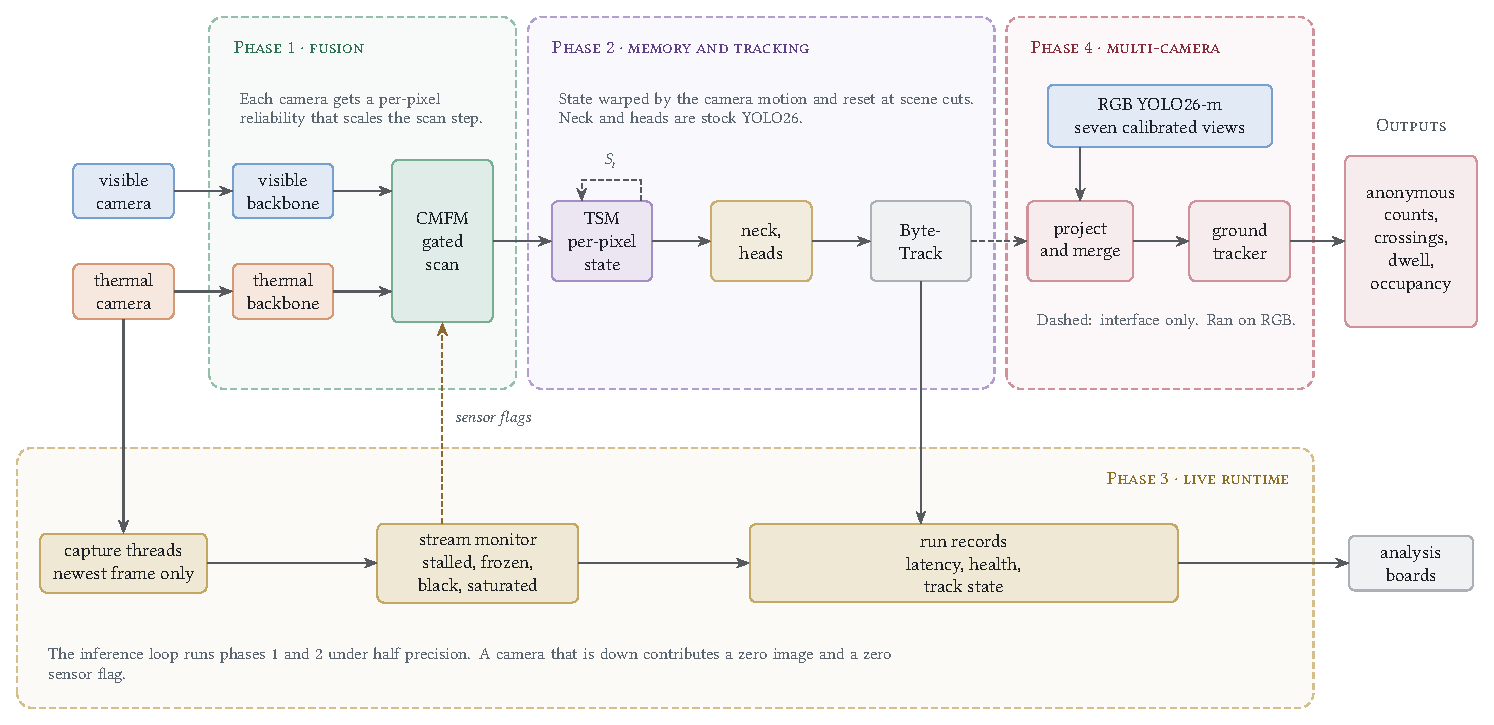
\includegraphics[width=0.92\textwidth]{figures/fig_pipeline.pdf}
\caption{The complete system. Paired visible and thermal cameras pass through the reliability-gated fusion detector, the Temporal State Memory and ByteTrack, inside a live runtime whose stream monitor raises sensor flags. The multi-camera ground-plane layer was run on an RGB-only detector, so its link from the tracker is the interface only.}
\label{fig:pipeline}
\end{figure*}

\begin{figure*}[!t]
\centering
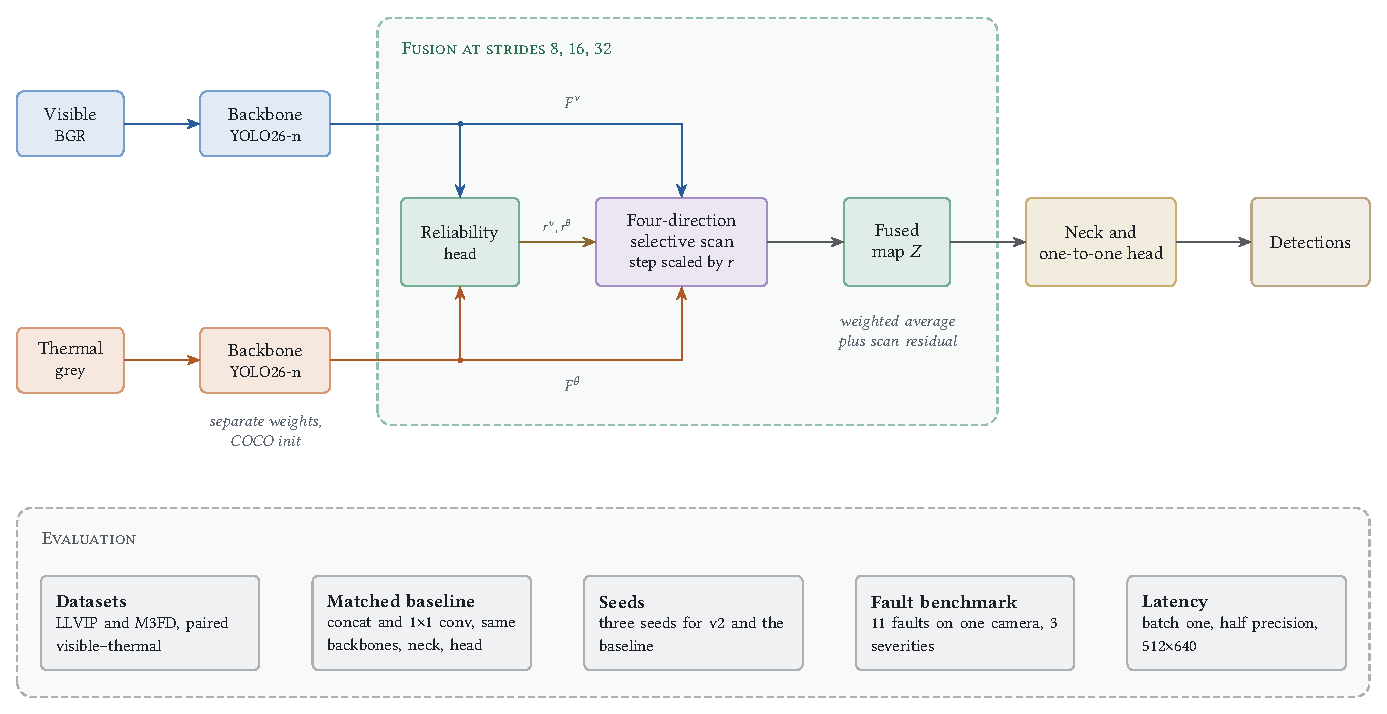
\includegraphics[width=0.92\textwidth]{figures/fig_phase1.pdf}
\caption{The fusion detector on still image pairs. Two YOLO26-n backbones feed a fusion block at strides 8, 16 and 32, in which a reliability head scales the step of a four-direction selective scan. The strip below lists the evaluation of the main paper.}
\label{fig:phaseone}
\end{figure*}

\begin{figure*}[!t]
\centering
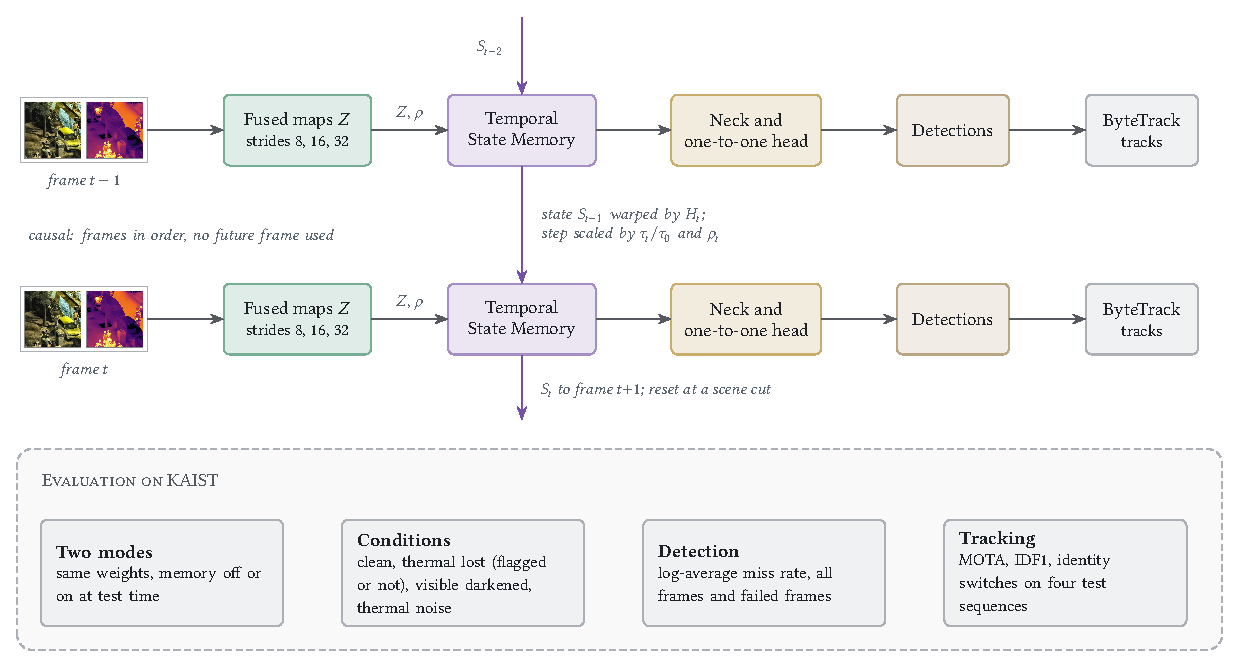
\includegraphics[width=0.92\textwidth]{figures/fig_phase2.pdf}
\caption{Video, the Temporal State Memory and tracking. The fused features of each frame update a per-pixel state carried from frame $t-1$ to frame $t$, warped by the homography and gated by elapsed time and reliability. Detections feed ByteTrack, and KAIST is scored with the memory off and on.}
\label{fig:phasetwo}
\end{figure*}

\begin{figure*}[!t]
\centering
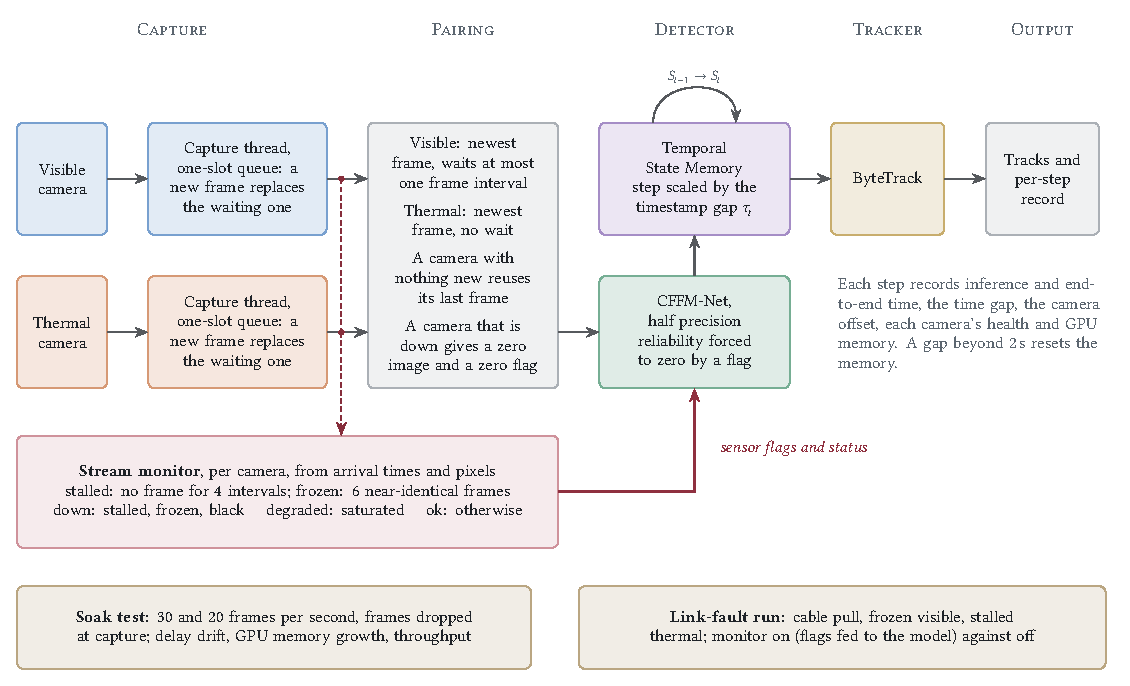
\includegraphics[width=0.92\textwidth]{figures/fig_phase3.pdf}
\caption{The live runtime. Two threaded captures with one-slot queues feed a newest-frame pairing step, then the detector with its memory and ByteTrack. A stream monitor watches each camera and feeds sensor flags back to the detector.}
\label{fig:phasethree}
\end{figure*}

\begin{figure*}[!t]
\centering
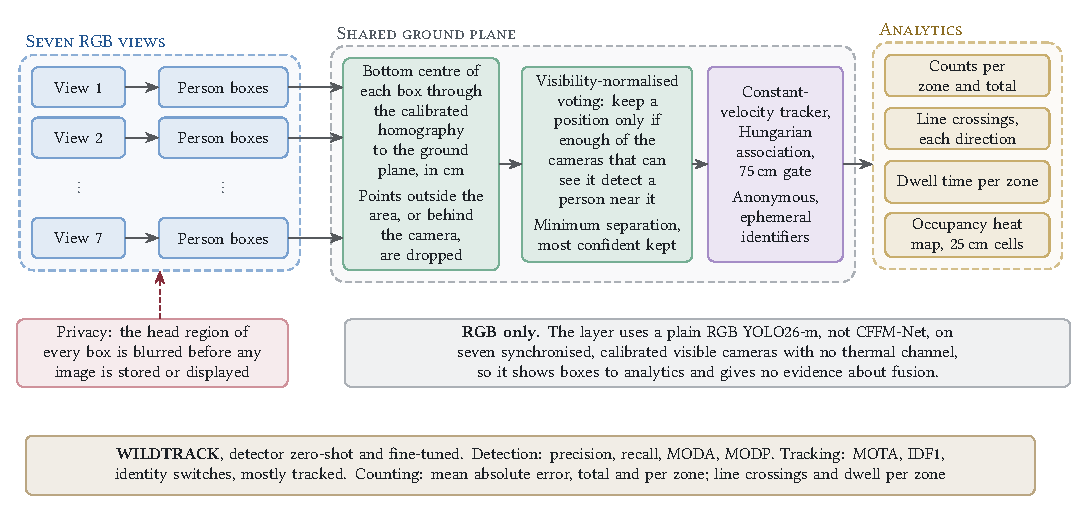
\includegraphics[width=0.92\textwidth]{figures/fig_phase4.pdf}
\caption{The multi-camera layer. Person boxes from each RGB view are projected to a shared ground plane, merged across cameras and tracked anonymously, giving counts, line crossings, dwell time and an occupancy map on WILDTRACK. The layer is RGB-only and gives no evidence about fusion.}
\label{fig:phasefour}
\end{figure*}
